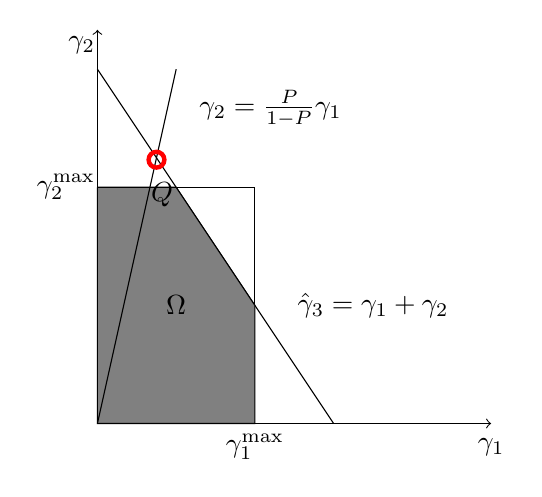
\begin{tikzpicture}
	\draw[<->] (0,5) -- (0,0) --(5,0);
	\draw (0,0) rectangle (2,3);
	\draw (3,0) -- (0,4.5);
	\draw[fill=gray] (0,0)--(0,3) to (0,0) -- (2,0) to (2,0)--(2,1.5) to (2, 1.5)--(1,3) to (0.58,3)--(0,3) ;
	\draw (0,0) -- (1,4.5);
	\draw[ultra thick, red](0.75,3.35) circle (0.1);
	\node (below) at (5,-0.3) {$\gamma_1$};
	\node (below) at (2,-0.3) {$\gamma_1^{\max}$};
	\node (left) at (-0.2,4.8) {$\gamma_2$};
	\node (left) at (-0.4,3) {$\gamma_2^{\max}$};
	\node (right) at (3.5,1.5) {$\hat{\gamma}_3=\gamma_1+\gamma_2$};
	\node (above) at (1,1.5) {$\Omega$};
	\node (right) at (2.2,4) {$\gamma_2=\frac{P}{1-P}\gamma_1$};
	\node (below) at (0.82,2.9) {$Q$};
\end{tikzpicture}